\subsection{Lift-Off}
\label{sec:fab:liftoff}

% \hl{9.375\% Describe the concept of the lift-off process, using schematics as required. [150 words max + Figures]}

Once the resist has been exposed and developed and the metallisation steps have been completed, the remaining resist can be stripped leaving the desired metal patterns. The metal on the top of the resist will be removed alongside the resist, and the metal in contact with the substrate will remain. Figure \ref{fig:lift-off} demonstrates this graphically.

\begin{figure}[!htb]
  \centering
  \begin{subfigure}[t]{0.5\textwidth}
      \centering
      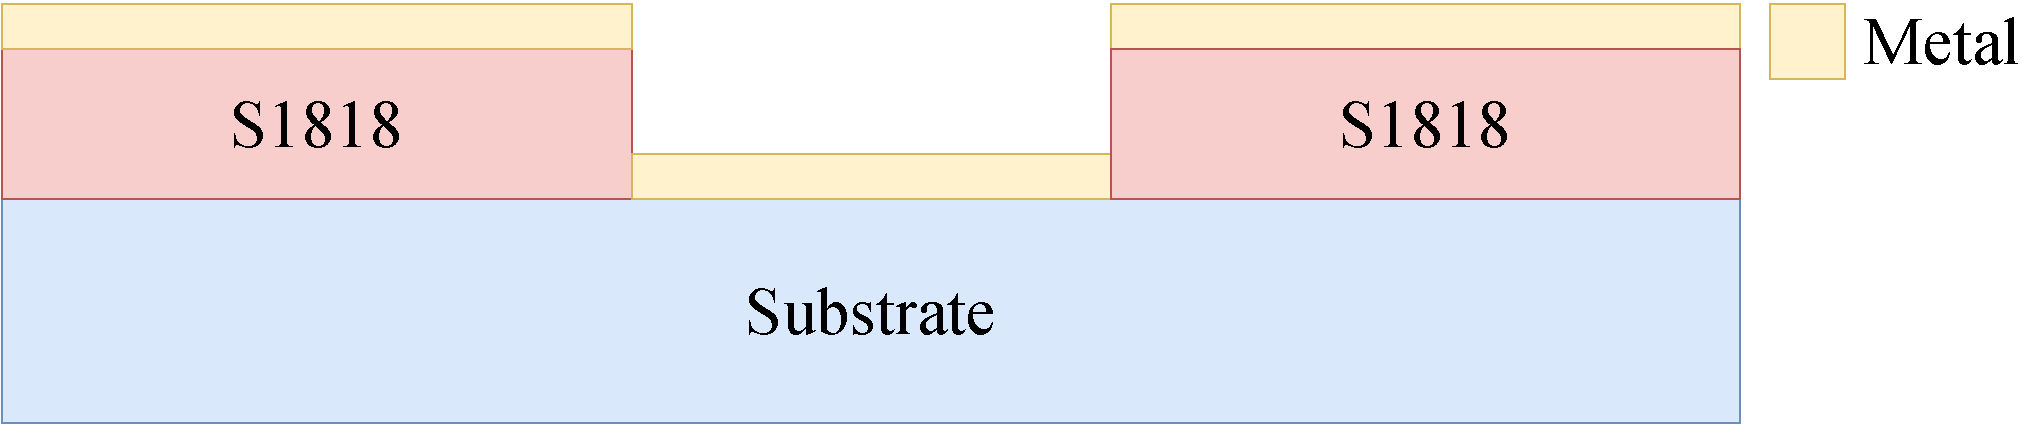
\includegraphics[width=0.95\textwidth]{Figures/angus_bruce/lift_off_microandnano1.pdf}
      \caption{Developed photoresist with metal deposition completed.}
  \end{subfigure}%
  ~
  \begin{subfigure}[t]{0.5\textwidth}
      \centering
      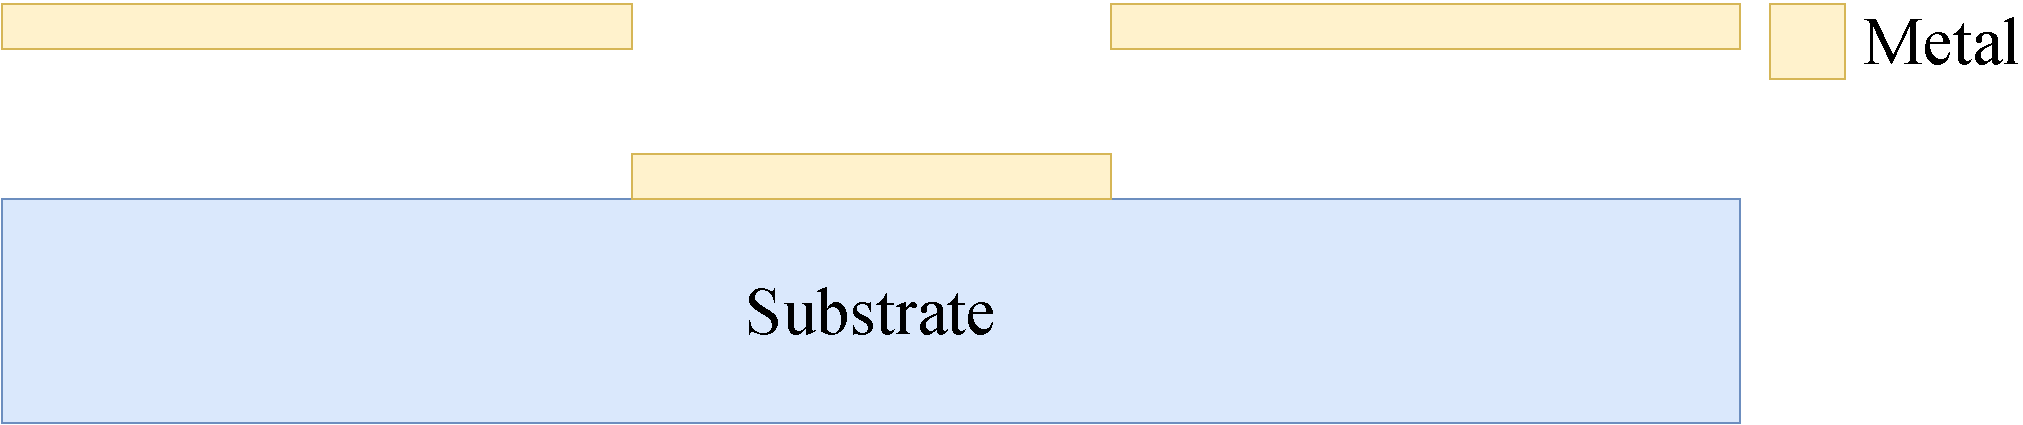
\includegraphics[width=0.95\textwidth]{Figures/angus_bruce/lift_off_microandnano2.pdf}
      \caption{Photoresist is dissolved undercutting the metal on top of it.}
  \end{subfigure}
  ~
  \begin{subfigure}[t]{0.5\textwidth}
      \centering
      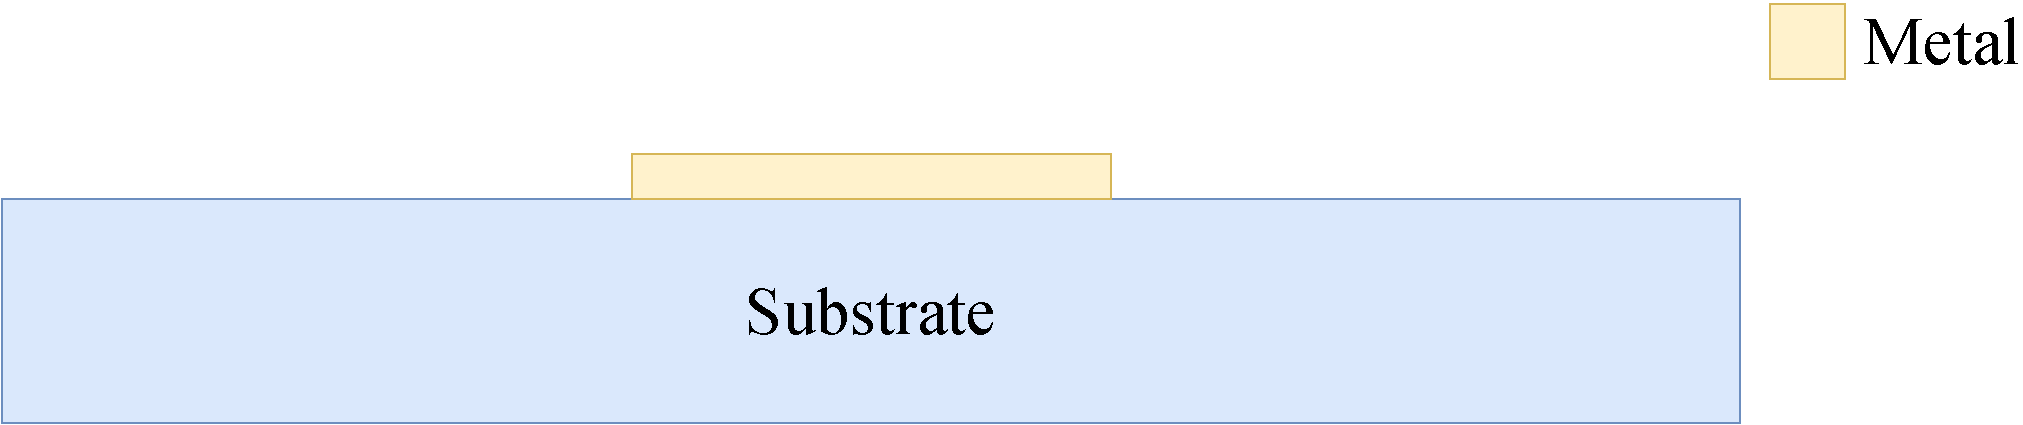
\includegraphics[width=0.95\textwidth]{Figures/angus_bruce/lift_off_microandnano3.pdf}
      \caption{Metal in contact with substrate remains.}
  \end{subfigure}
  \caption{Graphical representation of the lift-off process}
  \label{fig:lift-off}
\end{figure}

For this process, the substrate was placed in a beaker of acetone in a $50\degree C$ bath for a few hours to dissolve the undeveloped resist. It was then cleaned in IPA to remove any acetone residue.

% \hl{Suggest possible alternative process steps to achieve the same result as obtained in the lift-off process you have used. [50 words max]}

Either electron-beam lithography or a negative photoresist could also have been used to achieve the same metal pattern. E-beam would likely be unsuitable since the minimum feature size doesn't warrant it and if a negative photoresist process were to be used the photomask would need to be inverted.
